\documentclass{acm_proc_article-sp}


%\usepackage{scicite}
\usepackage{amsmath}

\usepackage{graphicx}
\usepackage{psfrag}
\usepackage{subfigure}
\usepackage[usenames]{color}
\usepackage[table]{xcolor}    % loads also colortb
\usepackage{array}
\usepackage{url}
\usepackage{amssymb}
\usepackage{natbib}
% \usepackage{amsthm}


\usepackage{times}

\renewcommand\ttdefault{aett}

  \long\def\remark#1{%
      \ifvmode
         \marginpar{\raggedright\hbadness=10000
         \parindent=8pt \parskip=2pt
         \def\baselinestretch{0.8}\tiny
         \itshape\noindent #1\par}%
      \else
          \unskip\raisebox{-3.5pt}{\rlap{$\scriptstyle\diamond$}}%
          \marginpar{\raggedright\hbadness=10000
         \parindent=8pt \parskip=2pt
         \def\baselinestretch{0.8}\tiny
         \itshape\noindent #1\par}%
      \fi}


\topmargin 0.0cm
\oddsidemargin 0.2cm
\textwidth 16cm 
\textheight 21cm
\footskip 1.0cm

\begin{document}

\title{MRFy: Remote Homology Detection for Beta-Structural Proteins
  Using Markov Random Fields and Stochastic Search}

\author{Noah M. Daniels \hspace*{8pt} Andrew Gallant \hspace*{8pt} Norman 
Ramsey \hspace*{8pt} 
Lenore Cowen\thanks{Corresponding author: lenore.cowen@tufts.edu}
\\ Department of Computer Science, Tufts University \\ 161 College Ave, 
Medford, MA 02155.}

\date{\today}

\maketitle



%%%%%%%%%%%%%%%%% END OF PREAMBLE %%%%%%%%%%%%%%%%

\begin{abstract}


\end{abstract} 

%%%%%%%%%%%%%%%%%%%%%%%%%%%%%%%%%%%%%%%%%%%%%%%%%%%%%%%%%%%%%%%%%%%%%%%%%%%%%%%%
%%%%%%%%%%%%%%%%%%
% BEGIN MAIN TEXT
%%%%%%%%%%%%%%%%%%%%%%%%%%%%%%%%%%%%%%%%%%%%%%%%%%%%%%%%%%%%%%%%%%%%%%%%%%%%%%%%
%%%%%%%%%%%%%%%%%%



\section{Introduction}

Recognition of remote homologs from protein sequence is a challenging
problem, particularly for beta-structural motifs, where many of the
residues whose interactions drive the fold can be a long way, and
variable distance apart in sequence. 
Many of the popular
sequence-based methods for recognizing close homologs, such as Profile
Hidden Markov Models (HMMs)~\cite{blah,blah}, perform particularly poorly on
$\beta$-structural motifs, precisely because the HMM model is not
powerful enough to capture these long-range dependencies~\cite{blah}. 
Several ways
to generalize these HMMs to Markov random fields (MRFs) have therefore
been proposed~\cite{blah,blah,blah}, but with the additional power of the 
random field comes several computational challenges. 
% comment by NMD: I find the following sentence extremely awkward,
% and we did not define "parse".
In particular, there is a tradeoff
between the complexity of the random field, and both the amount of
training data required, as well as the computational complexity of
computing the optimum parse of new sequences to the model.


In 2010, Menke, Berger and Cowen introduced
SMURF)~\cite{Menke:2010ti}, a Markov Random Field method designed to
recognize protein sequences that would fold into beta-propeller
shapes. 
While SMURF greatly improved beta-propeller recognition over
existing HMM and threading methods, it was actually quite simple as
far as MRFs are concerned: it combined a score based on a standard profile 
hidden Markov model with a conditional probability score that incorporated
the statistical preferences of the amino acid residues that are
hydrogen-bonded in $\beta$-sheets, thereby capturing some of the
strongest long-range dependencies in beta-structural motifs.
The
pairwise statistical preferences were learned from solved
$\beta$-structures across the entire PDB, so there was sufficient
training data. 
However, there was a great computational cost: the
minimum energy parse of the sequence to the Markov Random Field model
was generated exactly using a doubly-exponential multi-dimensional
dynamic program.


This computational cost was the barrier that prevented the SMURF MRF
from being applied directly to other $\beta$-structures, beyond just
the propellers.  
When run on $\beta$-barrels, or other $\beta$-structures with
even moderately complex strand interleaving patterns, the exact
computation of the SMURF MRF became completely intractable. 
There are two ways to approach this computational bottleneck. 
One is to simplify the random field, and only consider some of the pairwise 
statistical preferences for the beta-strands that are more local in sequence.
This is the approach we took in a 2012 paper of Daniels, Hosur, Berger
and Cowen, when we designed SMURFLite~\cite{Daniels:2012dg}. 
The other approach would be to retain the entire SMURF MRF, but consider
stochastic search approaches to heuristically explore parses of the
sequence to the MRF, in order to find low-energy but not necessarily
minimum-energy parses.
This is the approach we take in the present work.

In particular, we introduce MRFy, a suite of methods to perform
stochastic searches of the SMURF MRF. 
We show that MRFy, combined with Kumar and Cowen's {\em simulated evolution\/} 
outperforms HMMer (a popular HMM method), RaptorX (a state-of the art threading 
method), and HHPred (a profile-profile HMM method that has performed well at 
recent CASP competitions) at recognizing different beta-barrel superfamilies
in a stringent leave-family-out cross validation experiment. 
MRFy is available for download at \url{http://mrfy.cs.tufts.edu}. 
It is written in the Haskell functional programming language; some details of 
implementation are further discussed in~\cite{Daniels:2012cm}.

Finally, we find the best approach is a hybrid combination of
SMURFLite and MRFy: we initialize the MRFy stochastic search from the
best sequence parse that SMURFLite can find, and then run the
stochastic search from there. On the same set of $\beta$-barrel superfamilies 
considered in \cite{Daniels:2012dg}, we show 
we  show a mean XX\% (median YY\%) improvement in Area Under 
Curve (AUC) for
$\beta$-structural motif recognition as compared to the SMURFLite results 
in~\cite{Daniels:2012dg}.
By these same benchmarks, we show a mean 5.5\% (median 16\%) improvement over
HMMER (\cite{Eddy:1998ut}) (a popular HMM method), a mean 29\% (median
16\%) improvement as compared to RAPTOR (\cite{Xu:2003p3417}) (a
well-known threading method), and a mean 13\% (median 14\%) improvement in AUC 
over HHPred (\cite{Soding:2005ff}) (a profile-profile HMM method).



\section{Methods}

\subsection{Markov random field model}

MRFy builds on the SMURF and SMURFLite Markov random field 
model~\cite{Daniels:2012dg}, which uses multidimensional 
dynamic programming to simultaneously capture both standard HMM models and the
pairwise interactions between amino acid residues bonded together in
$\beta$-sheets. 

In particular, the ``Plan7'' hidden Markov model is modified to represent
hydrogen-bonded $\beta$-strands with additional, non-local edges.
Because the $\beta$-strands in a SMURF or MRFy template represent 
\emph{consensus} 
$\beta$-strands, those present in at least some fraction (in our experiments, 
at least
half) of the sequences participating in the training alignment, we prohibit
insertions and deletions in those strands.
Thus, we collapse those nodes of the ``Plan7'' model to be just match states;
the transitions to insertion and deletion states are removed.
Figure~\ref{mrfy_model} illustrates this architecture.


\begin{figure}[htb!]
\begin{center}
  \fbox{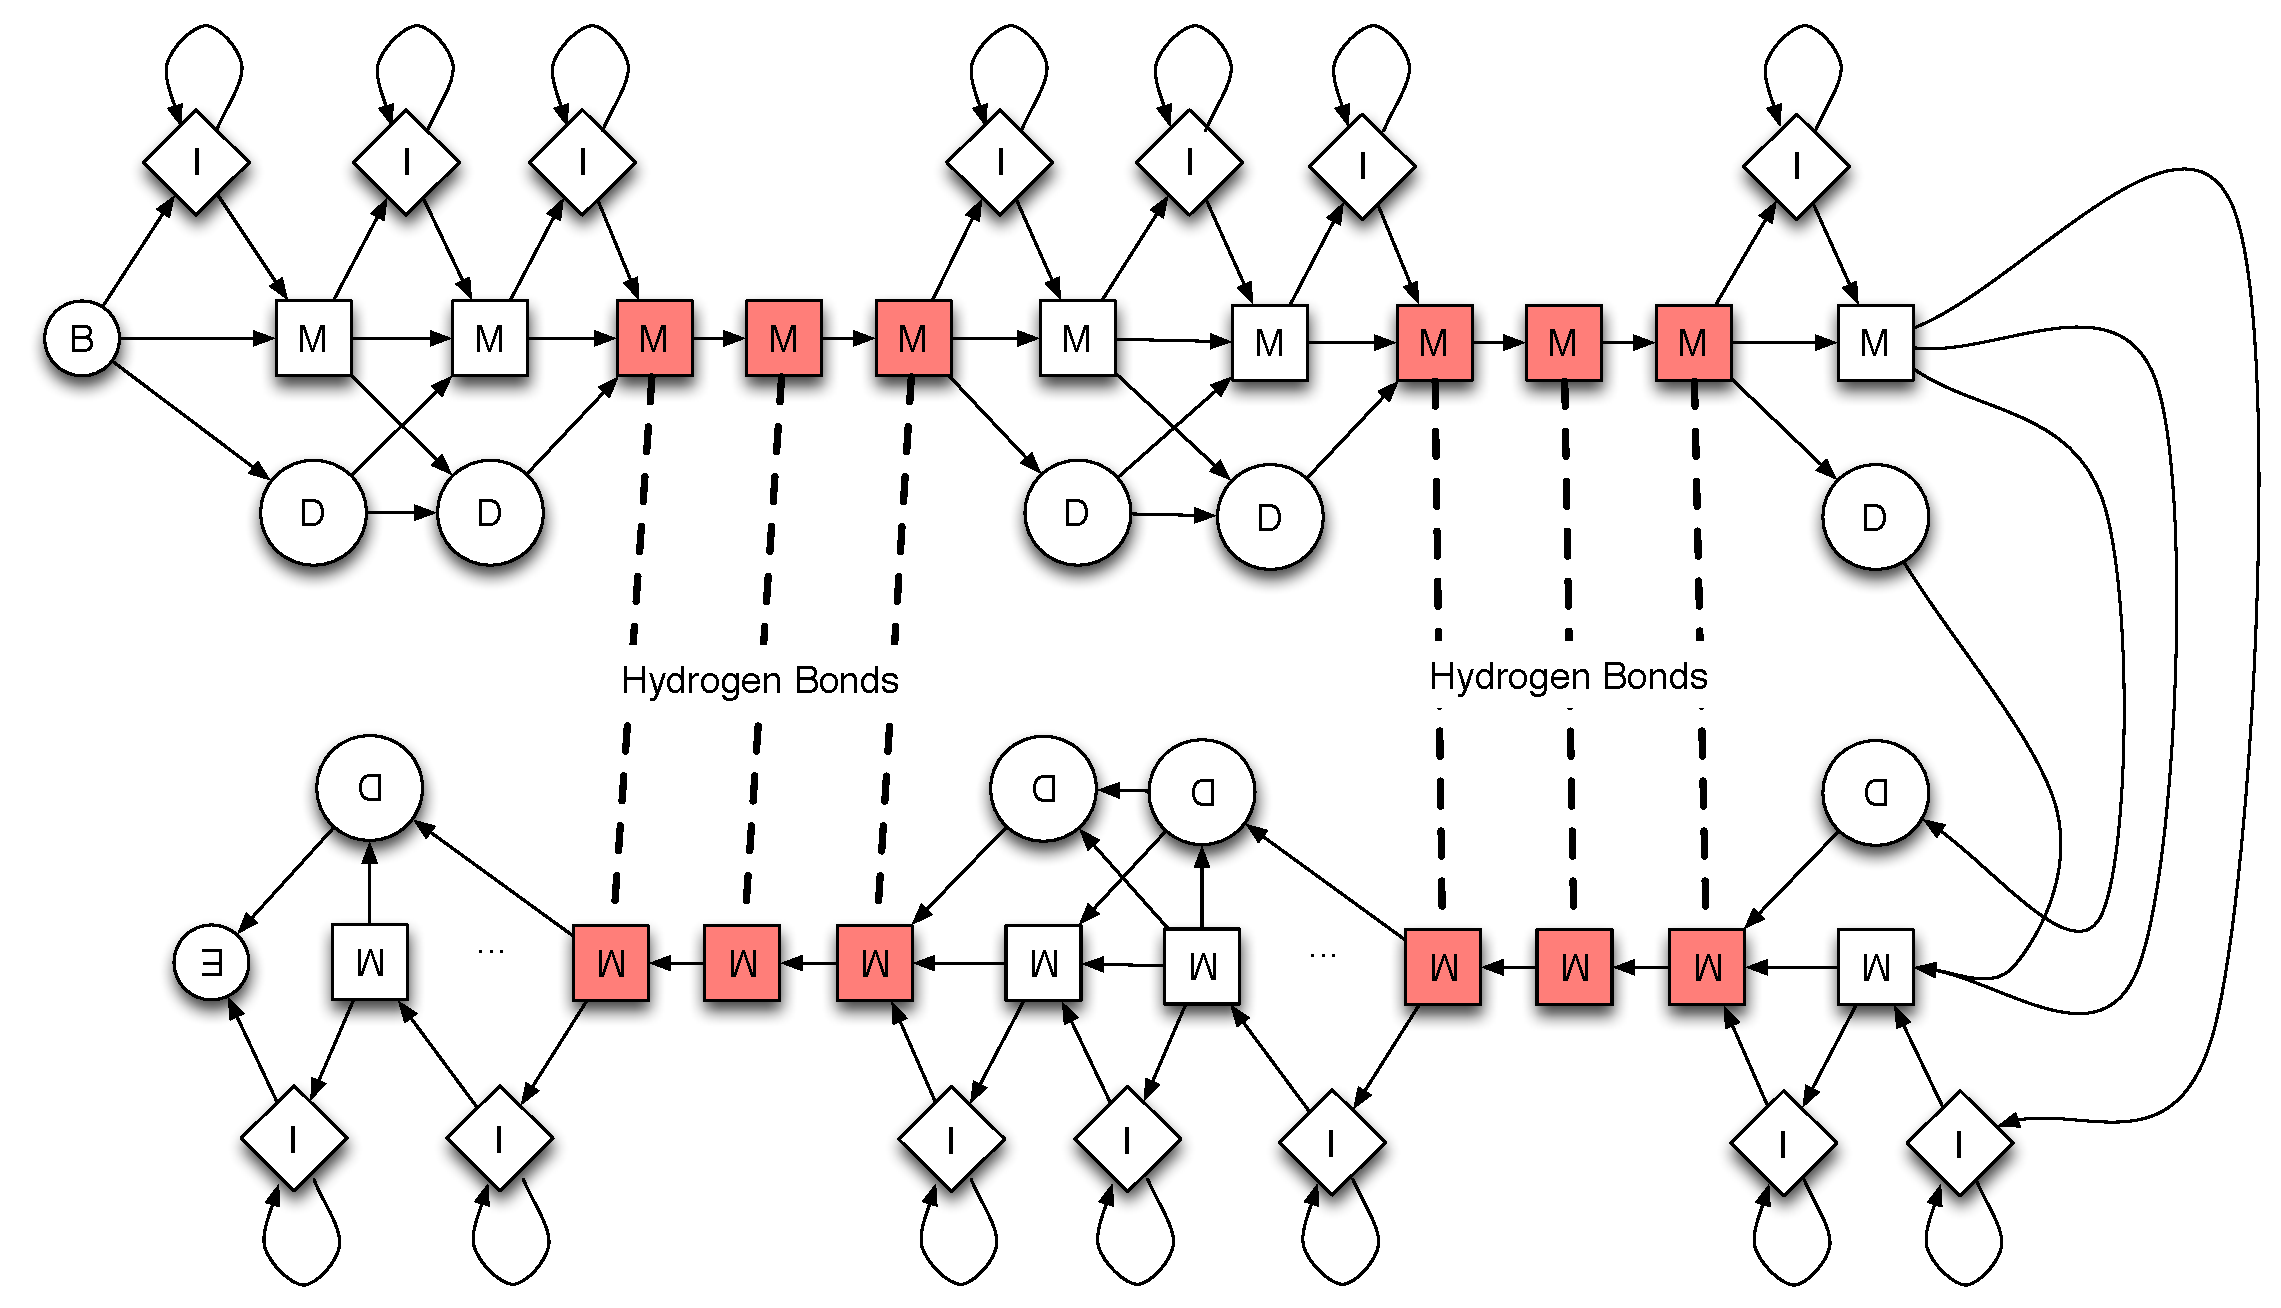
\includegraphics[width=2.8in]{mrf_interleave_diagram.pdf}}
   \caption{A MRFy Markov random field with two $\beta$-strand pairs}
   \label{mrfy_model}
 \end{center}
\end{figure}

The standard form of the Viterbi
recurrence relations for computing the most likely path of a sequence through
a hidden Markov model, as incorporated in HMMER~\cite{Eddy:1998ut} is:

\newcommand\txprobj[3][]{a#1_{{#2}_{j-1}{#3}_j}}
\newcommand\txprobjj[3][]{a#1_{{#2}_{j-1}{#3}_j}}
\newcommand\alignwidth{\ensuremath C} % number of columns in an alignment
\newcommand\pairedwith[1]{{\pi(#1)}}

\newcommand\vsum[2]{#2&{}+{}& #1}

\def\goo{18pt}
\def\gum{14pt}

\def\maxiquad{\hskip 1.2em\relax}
\begin{equation}
\begin{array}{@{}l@{}c@{}l}

V_{j}^{M}(i) &{}={}& \frac{e_{M_{j}}(x_{i})}{q_{x_{i}}} \times \max \left\{
  \begin{array}{l@{}c@{}l}
  V_{j-1}^{M}(i - 1) \times a_{M_{j-1}M_{j}}\\
  V_{j-1}^{I}(i - 1) \times a_{I_{j-1}M_{j}}\\
  V_{j-1}^{D}(i - 1) \times a_{D_{j-1}M_{j}}\\
  \end{array} \right.\\[\goo]
V_{j}^{I}(i) &=& \log\frac{e_{I_{j}}(x_{i})}{q_{x_{i}}} \times \max \left\{
  \begin{array}{l@{}c@{}l}
  V_{j}^{M}(i - 1) \times a_{M_{j}I_{j}}\\
  V_{j}^{I}(i - 1) \times a_{I_{j}I_{j}}\\
  \end{array} \right.\\[\gum]
V_{j}^{D}(i) &=& \max \left\{
  \begin{array}{l@{}c@{}l}
  V_{j-1}^{M}(i) \times a_{M_{j-1}D_{j}}\\
  V_{j-1}^{D}(i) \times a_{D_{j-1}D_{j}}\\
  \end{array} \right.\\

\end{array}
\end{equation}

In the SMURF or MRFy Markov random field model, we add non-local interactions 
to these
probabilities, resulting in conditional probabilities.
When column~$j$ of an alignment is part of a $\beta$-strand and is paired
with another column  $\pairedwith j$,
the probability of finding amino acid~$x_i$ in column~$j$ 
depends on whatever amino acid~$x'$  is in column~${\pairedwith i}$.
If~$x'$ is in position~$i'$ in the query sequence, Viterbi's
equations are altered; for example,
$V_{j}^{\prime M}(i)$ depends not only on
$V_{j-1}^{\prime M}(i-1)$ but also on
$V_{\pairedwith j}^{\prime M}(i')$.
The distance between $j$~and~$\pairedwith j$ can be as small as a few
columns or as large as a few hundreds of columns.
Because $V_j^{\prime M}(i)$~depends not only on nearby values but also on
$V_{\pairedwith j}^{\prime M}(i')$,
we must modify the Viterbi recurrence relations.

Note that hydrogen-bonded $\beta$-strand residues may only occupy match states 
in the Markov random field, so only the corresponding terms of the recurrence
relation need be modified.
The revised Viterbi recurrence relation for the Markov random field is:
\begin{small}
\begin{equation}
\begin{array}{@{}l@{}c@{}l}

V_{j}^{M}(i) &{}={}& \frac{e_{M_{j}}(x_{i})}{q_{x_{i}}} \times \max \left\{
  \begin{array}{l@{}c@{}l}
  V_{j-1}^{M}(i - 1) \times a_{M_{j-1}M_{j}} \times P(x_{i}|x_{\pi j})\\
  V_{j-1}^{I}(i - 1) \times a_{I_{j-1}M_{j}} \times P(x_{i}|x_{\pi j})\\
  V_{j-1}^{D}(i - 1) \times a_{D_{j-1}M_{j}} \times P(x_{i}|x_{\pi j})\\
  \end{array} \right.\\[\goo]

\end{array}
\end{equation}
\end{small}

where $x_{\pi j}$ represents the amino acid in column $\pi j$, which is 
hydrogen-bonded to the amino acid $x_{i}$ in column $j$.

For reasons of convenience, as well as avoiding floating-point underflow due to
exceedingly small numbers, we typically work in negative log space.
Since a probability can range from 0 to 1, the log of a probability must be a
negative number, and thus the negative log of that probability is a (small)
positive number.
Each probability is transformed into its negative log, resulting in the final
form:

\begin{small}
\begin{equation}\label{viterbi-final}
\begin{array}{l@{}c@{}l@{}}
V_{j}^{\prime M}(i) &=& e^{\prime}_{M_{j}}(x_{i}) + \min \left\{
  \begin{array}{l@{}c@{}l}
  \vsum{V_{j-1}^{\prime M}(i-1)} {a^{\prime}_{M_{j-1}M_{j}}} + P'(x_{i}|x_{\pi j})\\
  \vsum{V_{j-1}^{\prime I}(i-1)} {a^{\prime}_{I_{j-1}M_{j}}} + P'(x_{i}|x_{\pi j})\\
  \vsum{V_{j-1}^{\prime D}(i-1)} {a^{\prime}_{D_{j-1}M_{j}}} + P'(x_{i}|x_{\pi j})\\
  \end{array} \right.\\\\
V_{j}^{\prime I}(i) &=& e^{\prime}_{I_{j}}(x_{i}) + \min \left\{
  \begin{array}{l@{}c@{}l}
  \vsum{V_{j}^{\prime M}(i - 1)} {a^{\prime}_{M_{j}I_{j}}}\\
  \vsum{V_{j}^{\prime I}(i - 1)} {a^{\prime}_{I_{j}I_{j}}}\\
  \end{array} \right.\\\\
V_{j}^{\prime D}(i) &=& \min \left\{
  \begin{array}{l@{}c@{}l}
  \vsum{V_{j-1}^{\prime M}(i)} {a^{\prime}_{M_{j-1}D_{j}}}\\
  \vsum{V_{j-1}^{\prime D}(i)} {a^{\prime}_{D_{j-1}D_{j}}}\\
  \end{array} \right.\\
\end{array}
\end{equation}
\end{small}

given the transformations:

\begin{equation}
  \begin{array}{l@{}c@{}l@{}}
  a'_{s \hat{s}} = - \log a_{s \hat{s}} \\
  e^{\prime}_{s}(x) = - \log\frac{e_{s}(x)}{q_{x}}\\
  V_j^{\prime M}(i) = - \log V_j^{M}(i)\\
  P^{\prime}(x_{i}|x_{\pi j}) = - \log P(x_{i}|x_{\pi j})
  \end{array}\\
\end{equation}


This is exactly the recurrence relation that SMURF~\cite{Menke:2010ti} and 
SMURFLite~\cite{Daniels:2012dg} solve using multidimensional dynamic 
programming.
As demonstrated by Daniels, et al.~\cite{Daniels:2012dg}, as the 
\emph{interleave} 
of the $\beta$-strands increases, the computational complexity grows 
exponentially.

As an alternative to solving these more complex recurrence relations, we might
consider a divide-and-conquer approach.
Each $\beta$-strand can be thought of as breaking the larger model into two 
smaller
models; collectively, all the $\beta$-strands divide the Markov random field 
into many small, \emph{independent} hidden Markov models.
Thus, for any particular path through the Markov random field, corresponding to
a particular placement of query sequence residues onto the nodes of the model,
we could compute the augmented Viterbi score by summing the Viterbi scores of
each smaller hidden Markov model, along with the contribution to the Viterbi
score from the $\beta$-strands.

Since only match states are allowed for $\beta$-strand residues, the 
contribution of each such residue is only:

\begin{equation}
% \begin{split}
  \begin{array}{@{}l@{}c@{}l}
  V_{j}^{\prime M}(i) = e^{\prime}_{M_{j}}(x_{i}) + 
  \vsum{V_{j-1}^{\prime M}(i - 1)} {a^{\prime}_{M_{j-1}M_{j}}} + P(x_{i}|x_{\pi j})
  \end{array}
% \end{split}
\end{equation}

The asymptotic complexity of the Viterbi algorithm is $O(mn)$, where $m$ is the
length of the model and $n$ is the length of the query sequence.
Furthermore, the asymptotic complexity of the beta-strand contribution to the
Viterbi score for a particular placement of residues is just $O(b)$, where $b$
is the combined length of the $\beta$-strands.

Thus, a new algorithm for computing the optimal path through a Markov random 
field for a given query sequence presents itself.
Since we require that every $\beta$-strand position be occupied by a residue 
(as we force those positions into match states), we could simply consider every
possible assignment of a residue to a $\beta$-strand, computing the score for 
each one, and choose the best-scoring placement.

Metaphorically, we can picture the residues of the query sequence as beads,
and the Markov random field as the string of a necklace.
The $\beta$-strands can be thought of as particular substrings of the string 
that
must be covered by beads, while non-$\beta$ regions may be exposed (resulting in
delete states in the model).
To continue the metaphor, we may jam extra beads onto non-$\beta$ regions of the
string, resulting in insert states in the model.
Given that the beads already have a specified order, we must consider all the
ways to slide the beads up and down the string such that all of the 
$\beta$-regions
are covered.
Since the regions between $\beta$-strands can have their contribution to the
score computed according to the Viterbi recurrence relations, we need only
consider all the unique ways to assign residues to the $\beta$-strand nodes.

However, it is easy to show that there are an exponential number of such
assignments.

Let a Markov random field model $(N,B)$ be defined as a sequence $N$ of nodes 
$n_{i}, i \in (1..m)$, and a sequence $B$ of $\beta$-strands 
$b_{i}, i \in (1..k)$.
Each $\beta$-strand has length $l_{i}$, and contains a subsequence of the nodes
$N$.
This subsequence is determined by the
specifics of the model, which can be referred to as $b_{ij}, i \in (1..m), j \in
(1..l_{i})$.
Let a query sequence be defined as a sequence $R$ of residues
$r_{i}, i \in (1..n)$.
Let $L = \displaystyle \sum \limits_{i, i <= k} l_{i}$.

There are:
\begin{equation}
  \prod_{i \in (1..k)}{n - L - (i \times l_{max})} = 
  (n - 2L - k\times(l_{max}))^{\lceil \frac{k}{2} \rceil}
\end{equation}
possible placements of $R$ onto $(N,B)$.
Asymptotically, as $n$ grows, this is dominated by $n^k$, leading to an
asymptotic complexity of $O(n^k)$.

% \subsection{Proof that the model is exponential in complexity}\label{mrfy-proof}
% 
% Here, we prove that there are an exponential number of possible $\beta$-strand
% placements that must be considered.
% 
% \newdef{definition}{Definition}
% \begin{definition}
% Let a Markov random field model $(N,B)$ be defined as a sequence $N$ of nodes 
% $n_{i}, i \in (1..m)$, and a sequence $B$ of $\beta$-strands 
% $b_{i}, i \in (1..k)$.
% Each $\beta$-strand has length $l_{i}$, and contains a subsequence of the nodes
% $N$.
% Each $\beta$-strand contains an ordered sequence of nodes, determined by the
% specifics of the model, which can be referred to as $b_{ij}, i \in (1..m), j \in
% (1..l_{i})$
% Let a query sequence be defined as a sequence $R$ of residues
% $r_{i}, i \in (1..n)$.
% \end{definition}
% 
% \newtheorem{theorem}{Theorem}
% \begin{theorem}
% Given a model $(N,B)$ and a query sequence $R$, 
% $\displaystyle \sum \limits_{i, i <= k} l_{i}$ residues are placed in 
% $\beta$-strands.
% \end{theorem}
% 
% \begin{proof}
% Because each $\beta$-strand $b_{i}$ must be populated by exactly $l_{i}$ 
% residues,
% $\forall j, j > 1$, $b_{ij}$ is uniquely determined by the sequence $R$.
% For each $\beta$-strand position $b_{ij}$, one residue is placed.
% Thus, $\displaystyle \sum \limits_{i, i<=k} l_{i}$ residues are placed in 
% $\beta$-strands.
% \end{proof}
% 
% 
% \begin{definition}
%   Let $L = \displaystyle \sum \limits_{i, i <= k} l_{i}$.
% \end{definition}
% 
% 
% \begin{theorem}
% For a Markov random field $(N,B)$ with $k$ $\beta$-strands $b_{i}$, each of 
% length $l_{i}$, and thus containing positions for residues $b_{ij}$ and a query 
% sequence $r{i}$ of length $n$, there are $O(n^{k})$ ways
% to assign residues to the $\beta$-strands.
% \end{theorem}
% 
% 
% \begin{proof}
% Given that $L$ residues must be placed on $\beta$-strands, out of $n$ residues
% in the query sequence $R$, we can represent the problem as one of choosing
% an index $i \in (1..n)$ for the first position $b_{i1}$ of each $\beta$-strand.
% Since each $\beta$-strand $b_{i}$ consumes $l_{i}$ residues, this choice
% for the first $\beta$-strand, $b_{11}$, leaves $n - L - l_{i}$ possible 
% placements for $b_{21}$.
% In practice, $\beta$-strands range from two to twelve residues, so without loss 
% of generality, and to simplify counting, assume each $l_{i}$ is simply a
% maximum length $l_{max}$.
% Then choosing an index to place on $b_{i1}$, in general, leaves $n - L - 
% (i \times l_{max})$ choices for $b_{(i+1)1}$.
% Thus, there are:
% \begin{equation}
%   \prod_{i \in (1..k)}{n - L - (i \times l_{max})} = 
%   (n - 2L - k\times(l_{max}))^{\lceil \frac{k}{2} \rceil}
% \end{equation}
% possible placements of $R$ onto $(N,B)$.
% Asymptotically, as $n$ grows, this is dominated by $n^k$, leading to an
% asymptotic complexity of $O(n^k)$.
% \qed
% \end{proof}

A typical Markov random field might have 10 or 20 $\beta$-strands, and a typical
protein query sequence might have between 300 and 600 residues.
Thus, if we wish to consider all possible paths through a Markov random field
for a protein sequence, we must consider as many as 
$600^{10} \approx 6 \times 10^{27}$ possible paths through the model.

\subsection{Stochastic search}

Since an exhaustive search for an optimal alignment of a protein sequence to a
Markov random field is exponential in complexity, we turn to stochastic search
to mitigate this complexity.

Stochastic search encompasses a family of approaches for finding optimal or
near-optimal solutions to optimization problems.
Stochastic search approaches are promising when a search space is large, so that
exhaustive search is prohibitive, and when an optimization problem does not lend
itself to analytic solutions.
The generic form of stochastic search is that a solution is guessed at and 
evaluated, and then subsequent guesses are made as refinements to this initial
guess, until some termination condition is met.
The function used for evaluation is called the \emph{objective function}.

Framed as an optimization problem, MRFy, like SMURF, seeks to minimize the 
augmented Viterbi
score (see Equation~\ref{viterbi-final}), which equates to maximizing 
probability (recall that this score is the negative log of a probability).
SMURF~\cite{Menke:2010ti} finds this minimum exactly, using multi-dimensional dynamic programming,
which is exponential in the interleave number of beta strands.
MRFy, in contrast, uses stochastic search, as described next.

Given a placement of query-sequence residues into $\beta$-strand nodes of the
Markov random field, the score can be computed exactly.
Thus, the search space is the set of all possible ways to place residues on
these nodes..
Many stochastic search techniques rely on a gradient ascent (or descent)
approach, which makes moves (or refines guesses) along the steepest gradient,
leading quickly to local optima; various heuristics such as simulated 
annealing~\cite{Kirkpatrick:1983wa} can then help avoid getting stuck in poor
local optima.


However, we know of no way to compute a gradient on the search space of
$\beta$-strand placements, and so we must take approaches that do not rely
on this gradient.
Instead, we must rely on a random-mutation model of search, which generates one
or more candidate solutions (guesses) from a previous solution, and then
evaluates the cost function (in our case, the augmented Viterbi score) to
determine whether those guesses are better or worse than the previous step.
This can be likened to climbing a hill in the dark, feeling one's way with one 
foot before committing to a step.
This approach is referred to as \emph{random-mutation hill
 climbing}\cite{Davis:1991vx}.


In our representation, a particular solution is represented by an ordered list
of integers, one integer per $\beta$-strand in the Markov random field.
The value of each integer indicates the index, in the query sequence, of the
residue assigned to the first position of that $\beta$-strand.
Since the alignments to the regions of the Markov random field are solved
exactly by the Viterbi algorithm, this ordered list of integers uniquely
represents a solution to a Markov random field.

While the picture we have presented for our Markov random field model is most
precisely explained by assigning residue indices to the positions of 
$\beta$-strands, it may be more intuitive to consider the equivalent problem
of ``sliding'' these $\beta$-strands along the query sequence.
We will use this analogy in the following description of initial guesses.

We explored four models for generating initial guesses for our search
techniques:

\begin{itemize}
  \item \emph{Random-placement model}.
  First, we implemented a model that uniformly positions the $\beta$-strands
  along the query sequence, under the constraint that only legal placements
  may be generated, and thus the placement of any $\beta$-strand must leave 
  room for all the other $\beta$-strands in the model.
  
  \item \emph{Placement based on secondary structure prediction}.
  Next, we implemented a model that uses the PSIPRED~\cite{McGuffin:2000wx} secondary-structure
  prediction program to determine the positions of $\beta$-strands.
  Given a PSIPRED prediction for the secondary structure of a query sequence,
  we place $\beta$-strands at the most likely locations according to this
  prediction profile, randomized by a small amount of noise.
  The difficulty with this approach is that, while PSIPRED is reasonably 
  accurate when it is allowed to perform PSI-BLAST\cite{Altschul:1997tl} 
  queries to build a sequence
  profile, this comes at a run-time cost that completely dominates the running
  time of MRFy.
  However, while non-profile-based PSIPRED predictions are computationally 
  cheap, they provide poor accuracy.
  
  \item \emph{Placement based on scaling the template}.
  Third, we implemented a model based on the observation that true homologs
  to a structurally-derived template should have their $\beta$-strands in very
  roughly similar places, in sequence, to the proteins that made up that
  template.
  This will not always hold, but appears to provide for reasonable initial
  guesses.
  Given the position of each $\beta$-strand within a template Markov random 
  field, we scale the query sequence linearly (as it may be shorter or longer 
  than the model) and place the $\beta$-strands in scaled positions.
  Note that we do not scale the $\beta$-strands themselves; their lengths are
  preserved.
  We scale only the distances between $\beta$-strands.
  We inject a small amount of noise into the placements, so that 
  population-based models, such as multi-start simulated annealing and genetic
  algorithms, start with heterogenous solutions.
  
  \item \emph{Placement based on SMURFLite alignment}.
  Finally, we implemented a model that attempts to unify the SMURFLite and
  MRFy approaches.
  Given a template $T$, we create a new template, $T^\prime$, exactly as in
  \citet{Daniels:2012dg}, from which we have removed any $\beta$-strand pairs
  that exceed an interleave threshold of 2.
  We then run SMURFLite on $T^\prime$, to create an alignment $a^\prime$.
  Note that $a^\prime$ is an optimal solution to the template $T^\prime$.
  We wish to use $a^\prime$ as an initial guess for MRFy, but we must first add
  in the $\beta$-strands that were removed.
  In order to do so, we greedily move the placement of each $\beta$-strand in
  $a^\prime$ as needed to make room for those other $\beta$-strands.
  The resulting alignment $a$ becomes the initial guess for MRFy.
  
\end{itemize}

Since we do not know how to determine when a stochastic search process has found
a \emph{global} optimum (as opposed to a good local optimum), we must also have
some termination criterion for the search.
We implemented three alternative termination criteria:

\begin{itemize}
  \item A simple generation-counting approach, where the search terminates after
  a user-specified number of generations
  \item A time-based approach, where the search terminates after a 
  user-specified amount of time has elapsed
  \item A \emph{convergence} model, where the search terminates after the search
  has failed to improve after a user-specified number of generations
\end{itemize}
  
In practice, these criteria are easily combined, with a convergence approach
often halting searches early with good results, while the generation- or 
time-based limit ensuring that the search does not take longer than a user is
willing to wait.
We next describe the alternative heuristics that MRFy implements for stochastic
search: simulated annealing, a genetic algorithm, and a local search strategy.


\subsubsection{Simulated Annealing}

Simulated annealing~\cite{Kirkpatrick:1983wa} is a heuristic for stochastic search,
inspired by the physical process of annealing in metals.
Whereas a simple hill-climbing approach will always move downhill (if the task
is minimization) or uphill (if the task is maximization), if the search begins
near to a poor local optimum, the search will terminate at that local optimum.
Simulated annealing introduces an \emph{acceptance probability function}:
\begin{equation}
  \begin{split}
  P(e,e',T) = \begin{cases}
    1, & \text{ if } e' < e\\
    \exp(-(e'-e)/T),& \text{ otherwise }\\
\end{cases}\\
  \text{ where }
     e = E(s) \\
     e' = E(s')\\
  \end{split}
\end{equation}
which relies on some energy function $E(s)$ of the current state $s$ and
a candidate state $s'$, and a temperature function $T$ that tends towards zero
as the search progresses.
In our implementation, we used an exponentially-decaying temperature function:
\begin{equation}
  T(t) = k^{t}\times T_{0}
\end{equation}
given time $t$, initial temperature $T_{0}$, and a constant $k$.
The motivation for this decaying temperature function is that, as time 
progresses, the likelihood of being in a \emph{poor} local optimum lessens, and
thus, the closer to random hill-climbing we would like the search to behave.


Our energy function $E(s)$ is, naturally, the augmented Viterbi score of a
placement:
\begin{equation}
  E(s) = V_{m}^{\prime M}(n)
\end{equation}
where $m$ is the final residue in the query sequence and $n$ is the final
node in the Markov random field, and the $\beta$-strand placements are 
determined by $s$.

We implemented simulated annealing in MRFy according to this model.
We also implemented a \emph{multi-start} version of simulated annealing in MRFy,
where a set of independently-generated guesses is subject to simulated-annealing
random descent, in parallel.
At the termination of the search, the best solution from among all the 
candidates is chosen.


\subsubsection{Genetic Algorithm}

A genetic algorithm~\cite{Holland:1977hl} is a search heuristic inspired by 
biological evolution.
A genetic algorithm relies on the idea of \emph{selection} among a population of
varied solutions to an optimization problem.
At each of many generations, the fitter individuals in the population--those
solutions which exhibit more optimal scores--are allowed to continue into the
next generation.
Not only do they continue into the next generation, but they are allowed to
``reproduce,'' or recombine, to produce new solutions.
A particular solution to a problem, within the context of a genetic algorithm,
is called a \emph{chromosome}.
At each generation, some fraction of the fittest solutions are selected and
randomly paired with one another.
Each pair of solutions produces one or more offspring; each offspring is the
result of two steps: \emph{crossover} of the two chromosomes, followed by
random \emph{mutation} of the offspring.
The mutation is nondeterministic; the crossover may be deterministic or
nondeterministic.
The resulting offspring, along with their parents, are then evaluated according
to the objective function, and this process iterates until some termination
condition.


MRFy's genetic algorithm implementation uses the same representation for a
placement as simulated annealing: an ordered list of integers.

Let a \emph{placement} $p$ on a model with $k$ $\beta$-strands be an ordered 
set of integers $p_{i}, i \in (1..k)$.
Given two placements, $p$ and $q$, MRFy implements crossover of two chromosomes 
using the following algorithm:

\begin{enumerate}
  \item Set the new placement, $p'$, to the empty set.
  \item Repeat until all placements have been chosen:
  \begin{enumerate}
    \item Set the position for $p'_{0}$ to $p_{0}$
    \item Set the position for $p'_{k}$ to $q_{k}$
    \item Remove $p_{0}$, $p_{k}$, $q_{0}$, and $q_{k}$
    \item Adjust indices so $p$ and $q$ now range from what had been 1 to $k-1$.
  \end{enumerate}
\end{enumerate}

Our actual implementation is purely functional, and simply consumes elements 
from lists.
In effect, though, this algorithm simply chooses the `left-most' elements from 
one parent and the `right-most' elements from another.
After crossover, the mutation step simply moves each element $p_{i}$ of the
placement $p$ by a small, random amount, within the constraints imposed by the
neighboring $\beta$-strands.
The motivation behind this approach is to take two solutions that are of high
fitness (recall that the worst solutions at every generation are not allowed
to contribute to the next generation), and produce a new solution that combines
one ``half'' (roughly) of one solution with one ``half'' of the other.
See Figure~\ref{crossover} for an illustration of this procedure.

\begin{figure}[htb!]
\begin{center}
  \fbox{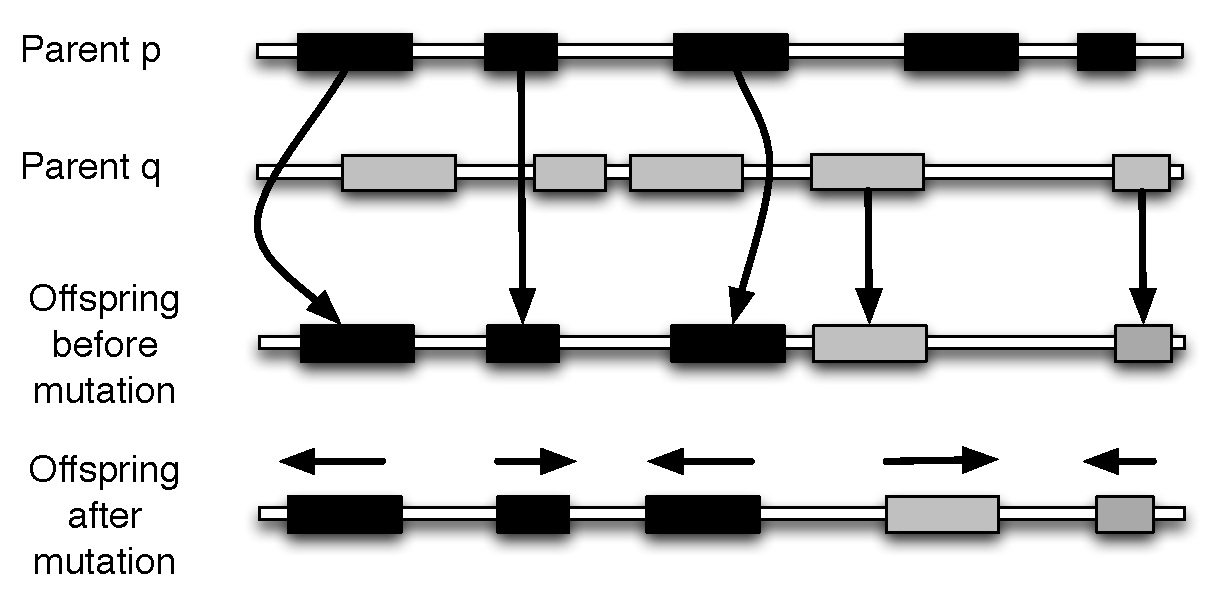
\includegraphics[width=2.8in]{crossover.pdf}}
   \caption{The crossover and mutation process in MRFy's genetic algorithm 
   implementation.
   Given parent $p$ (black) and parent $q$ (gray), alternate left and right
    placements from $p$ and $q$.
    Then, apply small random mutations to the resulting placement $p'$.}
   \label{crossover}
 \end{center}
\end{figure}


Given these operations for crossover and mutation, MRFy's genetic algorithm
implementation initializes a population of a user-specified size $P$ (typically 
one thousand placements, though we experimented with as many as ten thousand).
In parallel, each placement is scored according to the objective function.
Since scoring is far more computationally expensive than crossover and mutation,
we allow them all to reproduce, paired at random.
We then score them, and choose the $P$ best-scoring placements for the next
generation.
This process repeats until a termination condition is met, at which point the
single best placement is returned.
We note that a future enhancement to MRFy could return the $k$ best placements
for some user-specified threshold $k$, if multiple high-scoring alignments were
to be considered.


\subsubsection{Local Search}\label{localsearch}

Constraint-based local search~\cite{Hentenryck:2009vn} is a family of approaches
for exploring ``neighborhoods'' in feature space in a randomized manner, 
subject to the constraints of that solution space.
In the context of MRFy, the constraints are the previously-discussed 
restrictions that $\beta$-strands cannot overlap, and every residue must be
placed in a $\beta$-strand.
The motivation for local search is, in a particularly uneven
fitness landscape, hill climbing will often reach nearby local optima. Thus,
given a single candidate solution, local search explores the immediate 
neighborhood in great detail (perhaps, but not necessarily exhaustively).
When the local search cannot escape a local optimum, then some sort of 
\emph{non-local} move may be attempted.

This non-local move may rely on a population-based diversification approach,
in which parts of the solution may change dramatically.
In a sense, local search bears some resemblance to a genetic algorithm,
except that a population of solutions is created only when the search is stuck
in a local optima, and the best solution in that population is chosen for a new
search.

In MRFy's implementation, each step in the search consists of two phases: 
\emph{diversification} (See Figure~\ref{diversification}) and 
\emph{intensification}.
The diversification algorithm is as follows:
\begin{itemize}
\item Begin with a candidate solution $s$ (a placement), which is just
an ordered list of integers.
\item Given $s$, break the list into three sub-lists $s_{0}, s_{1}$, $s_{2}$, 
at randomly-chosen boundaries.
\item Choose one of the sub-lists $s_{i}$ at random, and mutate it into $k$ 
copies $s_{i1}$ through $s_{ik}$ at random, for some user-defined value of $k$ 
(we used $k=10$), within
the constraints imposed by the other sub-lists and the lengths of the 
$\beta$-strands.
\item Re-combine each set of lists, $(s_{1j}, s_{2j}, s_{3j})$ into a new 
placement $s^{\prime}_{j}, j \in (1..k)$.
\item Score each placement $s^{\prime}_{j}$, return the best-scoring of the $k$ new placements as a new solution.
\end{itemize}

Once diversification produces a new candidate solution, intensification brings
it toward a local maximum.
The intensification algorithm is as follows:
\begin{itemize}
\item Begin with a candidate solution $s$.
\item Repeat until no better-scoring placements are generated.
\begin{itemize}
  \item For each element $e \in s$, generate four new placements $s'_{i1}$ 
  through $s'_{i4}$ by moving $e$ up and down by 1 and two, as long as those 
  moves do not violate the constraints.
  \item Score each candidate placement $s'_{ij}$.
  \item Set $s$ to the best-scoring candidate placement $s'_{ij}$
\end{itemize}
\item Return $s$ as a new solution.
\end{itemize}

\begin{figure}[htb!]
\begin{center}
  \fbox{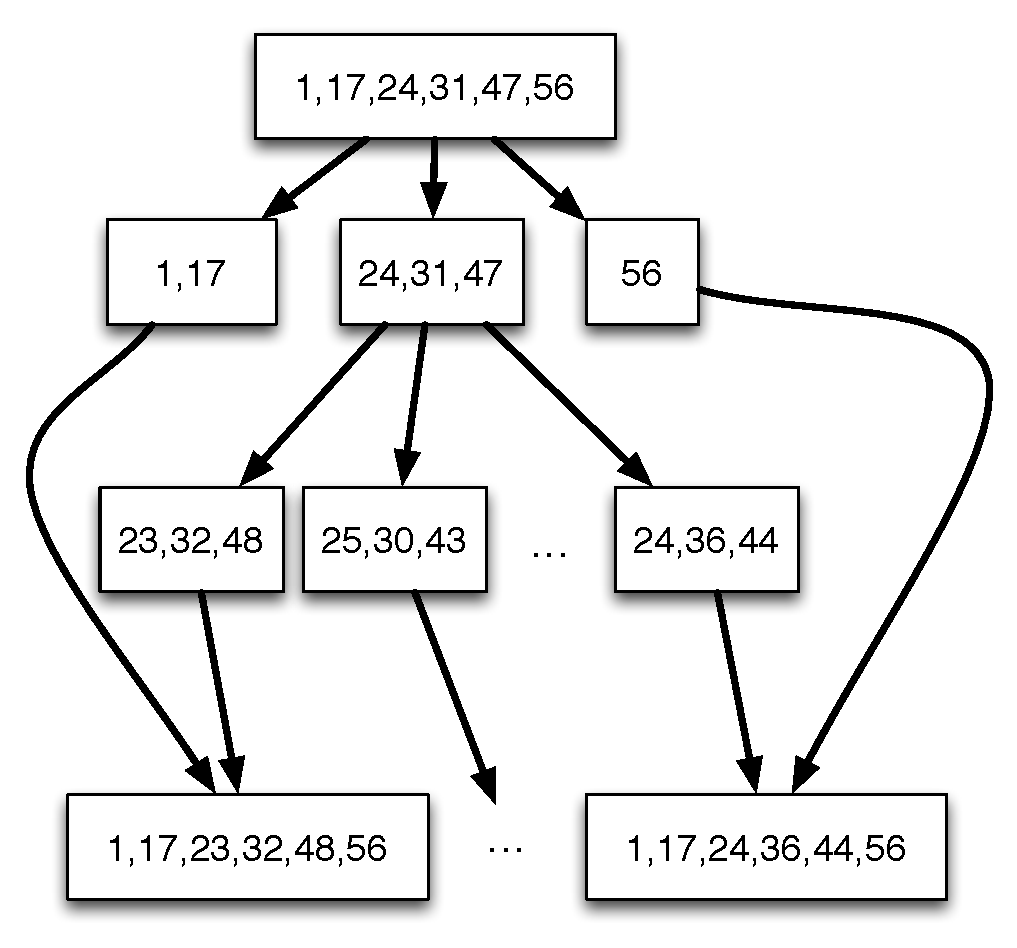
\includegraphics[width=2.8in]{localsearch.pdf}}
   \caption{The diversification step in local search.}
   \label{diversification}
 \end{center}
\end{figure}

% 
% These are from sandwich
% 
% [1,17,24,31,47,56,68,88,120,137,149,161,173,186,202,219,224] 554.4214648689649
% [1,17,24,31,47,56,68,88,120,128,136,140,150,160,202,219,224] 650
% 
% they can be divided as follows;
% [1,17,24,31,47,56,68,88,120] -> no change
% [128,136,140] -> 10 difference
% [150,160] -> 23 difference
% [202,219,224] -> No change

%%

\subsection{Evaluating search strategies}\label{searchstrats}

As MRFy supports three significantly different stochastic search strategies, and
a number of tunable parameters such as termination conditions and (for 
simulated annealing) the cooling schedule, we conducted a search over parameter
space using a small data set.
We built Markov random field templates from the fold ``8-bladed Beta-Propellers'', and the superfamilies ``Barwin-like endoglucanases'' (a 
$\beta$-barrel superfamily) and ``Concanavalin A-like lectins/glucanases'' (a 
$\beta$-sandwich superfamily).
We were interested in the speed of convergence for a true-positive test case,
so we tested each template with a protein sequence chosen from that fold or
superfamily: for the 8-bladed propeller, we chose ASTRAL chain d1lrwa\_
(Methanol dehydrogenase, heavy chain from  \emph{Paracoccus denitrificans}).
For the barwin-like endoglucanases, we chose ASTRAL chain d2pica1 
(Membrane-bound lytic murein transglycosylase A, MLTA from \emph{E. coli}).
For the lectins/glucanases, we chose ASTRAL chain d2sbaa\_ 
(Legume lectin from soy bean (\emph{Glycine max})).

We tested simulated annealing with a population size of 10, a maximum number of
generations of 10000, convergence periods of 200, 500, and 1000 generations, 
and a cooling factor of 0.99 (preliminary tests showed little impact from
varying the cooling factor among 0.9, 0.99, and 0.999).

We tested the genetic algorithm implementation with a population size of 1000 
and 10000, a maximum number of generations of 500, and convergence
periods of 10, 50, and 100.

Since the local search distinguishes between diversification and 
intensification, counting the number of generations is ambiguous; we used a time
limit of 10 seconds, 30 seconds and 5 minutes.
All tests were conducted on a 12-core AMD Opteron 2427 with 32GB RAM, devoting 
all 12 cores to MRFy.
For each test, we report statistics based on ten runs for each set of 
parameters.

\subsection{Simulated Evolution} \label{mrfy-simev}

In MRFy, we incorporated precisely the same ``simulated evolution'' 
implementation, as first proposed by Kumar and 
Cowen~\cite{Kumar:2009tp, Kumar:2010wv}, as we did for SMURFLite
in~\cite{Daniels:2012dg}.
We added pairwise mutations based on $\beta$-strand pairings.
Unlike in \citet{Daniels:2012dg}, 
here we were not attempting to mitigate
the loss of information due to simplifying the Markov random field, but rather
attempting to compensate for sparse training data.
This was motivated in part by the observation that SMURFLite benefited most
from simulated evolution when the ``number of effective families'' was low.
We use the same mutation frequencies as in \citet{Daniels:2012dg}.
For each artificial sequence, we mutate at a 50\% mutation rate per length of 
the $\beta$-strands. 

\subsection{Datasets} \label{mrfy-datasets}

From SCOP (\cite{Murzin:1995uh}) version 1.75, we chose the same
$\beta$-structural superfamiles as \citet{Daniels:2012dg}.
These superfamilies were: ``Nucleic acid-binding proteins'' (50249), 
``Translation proteins'' (50447), 
``Barwin-like endoglucanases'' (50685), ``Cyclophilin-like'' (50891), ``Sm-like 
ribonucleoproteins'' (50182), ``PDZ domain-like'' (50156), ``Prokaryotic 
SH3-related domain'' (82057), ``Tudor/PWWP/MBT'' (63748), ``Electron Transport 
accessory proteins'' (50090), ``Translation proteins SH3-like domain'' (50104), 
and ``FMN-binding split barrel'' (50475). 

\subsection{Training and testing process} \label{mrfy-training}

For the $\beta$-barrel superfamilies, we performed strict leave-family-out 
cross-validation. 
We built training templates at the superfamily level. 
For each superfamily, its constituent families were identified. 
Each family was left out, and a training set was established from the protein 
chains in the remaining families, with duplicate sequences removed. 
We built an MRF on the training set, both with and without training-data
augmentation using the same ``simulated evolution'' implementation as 
\citet{Daniels:2012dg}: we generate 150 new artificial training 
sequences from each original training sequence. 
For each artificial sequence, we mutate at a 50\% mutation rate per length of 
the $\beta$-strands.
We chose protein chains from the left-out family as positive test examples. 
Negative test examples were protein chains from all other superfamilies in SCOP 
classes 1, 2, 3 and 4 (including other barrel superfamilies), indicated as 
representatives from the nr-PDB (\cite{Berman:2000hl}) database with 
non-redundancy set to a BLAST E-value of $10^{-7}$.

We used MRFy's local search mode (see Section~\ref{localsearch}) to align each
test example to the trained MRF.
The score reported for MRFy was the combined HMM and pairwise score from the 
MRF, which is identical to the SMURF energy function.
For each training set, the scores for both methods (MRFy with and without
simulated evolution) were collected and a ROC curve (a plot of true positive 
rate versus false positive rate) computed. We report the area under the curve 
(AUC statistic) from this ROC curve (\cite{Sonego:2008uy}).



%%%%%%
\section{Results}

\subsection{Search strategies}

For the three stochastic search approaches, we compared the raw score achieved
by each approach under a variety of conditions, as discussed in 
Section~\ref{searchstrats}.
The raw score is simply the negative log of the probability of the best path
found through the model.
Thus, raw scores are not comparable between models, but they are comparable
between query sequences for a given model.

Table~\ref{ss-propeller} indicates the performance of different stochastic
search techniques on the 8-bladed $\beta$-propeller fold.
While the simulated annealing and genetic algorithm approaches exhibit less
variance (a smaller standard deviation) from run to run, they do not approach
the minimum score of the local search approaches. Multi-start simulated 
annealing with a population of 10 and a convergence threshold of 200 generations
averages 29.3 seconds per search, but only achieves a minimum score of 2112, 
though it converged in all cases.

In contrast, local search, given 30 seconds, achieves a minimum score of 1982, 
and even in only 10 seconds achieves a minimum score of 1992.
However, the global minimum score of 1781, which is achieved by SMURF on the
8-bladed $\beta$-propeller template, is only reached by MRFy with local search
two out of ten times, and this result required local search be allowed to run
for twenty minutes.
Thus, for this problem domain, local search seems to outperform our simulated
annealing and genetic algorithm implementations.


Table~\ref{ss-barwin} indicates the performance of the stochastic
search techniques on the ``Barwin-like endoglucanases'' $\beta$-barrel 
superfamily.
These structures are less complex than the propellers, even though they are
\emph{more} computationally complex for SMURFLite~\cite{Daniels:2012dg} if an 
interleave threshold greater than 2 is used. 
We see less variance than with the propellers, but once again, the local search
technique achieves a lower minimum score than simulated annealing or the genetic
algorithm.

Notably, local search achieves a minimum score of 978, which an 
\emph{exhaustive} search indicates to be a global minimum for this sequence on
this template.
With a time limit of 10 seconds, local search found this global minimum in one 
out of ten runs. 
With a time limit of 30 seconds, local search found it in two out of
ten runs, and with a time limit of 5 minutes, in four out of ten runs.

\rowcolors{2}{gray!25}{white}

\begin{small}
\begin{center}
\begin{table*}[htb]
\caption{Stochastic search performance on 8-bladed $\beta$-propeller \label{ss-propeller}}
\begin{tabular}{lllll}
\hline
             & Min Score & Mean Score & Std Score & Mean Time (s) \\
\hline
SA 200       & 2112      & 2139       & 12.2      & 29.3      \\
\hline                                                        
SA 500       & 2129      & 2146       & 9.3       & 1020      \\
\hline                                                        
SA 1000      & 2112      & 2130       & 7.8      & 3314      \\
\hline                                                        
GA 1000/10   & 2105      & 2126       & 6.6      & 285      \\
\hline                                                        
GA 1000/50   & 2094      & 2118       & 7.7      & 1239      \\
\hline                                                        
GA 1000/100  & 2107      & 2120       & \textbf{3.8}      & 548      \\
\hline                                                        
GA 10000/10  & 2087      & 2111       & 7.2      & 5809      \\
\hline                                                        
GA 10000/50  & 2094      & 2112       & 7.1      & 5174      \\
\hline                                                        
GA 10000/100 & 2079      & 2114       & 9.0      & 10226      \\
\hline                                                        
LS 10s       & 1992     & 2015      & 19.4     & \textbf{10}    \\
\hline                                                        
LS 30s       & 1982     & 1991      & 10.9     & 30    \\
\hline                                                        
LS 5m        & \textbf{1818}     & \textbf{1876}      & 37.2     & 300    \\
\hline
\end{tabular}\\
{Performance of stochastic search techniques on an 8-bladed $\beta$-propeller
template. SA is Simulated Annealing, GA is Genetic Algorithm, and LS is Local
Search. For Simulated Annealing, we show results for convergence thresholds of
200, 500, and 1000 generations. 
For the Genetic Algorithm, we show results for convergence thresholds of 10, 
50, and 100 generations, and for population sizes of 1000 and 10000.
For Local Search, we show results for time limits of 10 seconds, 30 seconds and 
five minutes, on a 12-core AMD Opteron.
MRFy never achieved the global optimum score of 1781, achieved by SMURF, on this
template, except when local search was given 20 minutes of compute time, in
which case it found the global optimum two out of ten times.}
\end{table*}
\end{center}
\end{small}

\begin{small}
\begin{center}
\begin{table*}[htb]
\caption{Stochastic search performance on ``Barwin-like'' $\beta$-barrel \label{ss-barwin}}
\begin{tabular}{llllll}
\hline
             & Min Score & Mean Score & Std Score & Mean Time (s) & Optimal \\
\hline
SA 200       & 1064      & 1071       & 3.8      & 79.5  & 0    \\
\hline                                                        
SA 500       & 1047      & 1063       & 7.6      & 104   & 0   \\
\hline                                                        
SA 1000      & 1024      & 1047       & 14.0      & 523  & 0    \\
\hline                                                        
GA 1000/10   & 1061      & 1069       & 3.6      & 232   & 0   \\
\hline                                                        
GA 1000/50   & 1059      & 1066       & 3.1      & 442    & 0  \\
\hline                                                        
GA 1000/100  & 1058      & 1069       & 4.0      & 1382   & 0   \\
\hline                                                        
GA 10000/10  & 1058      & 1063       & 2.5      & 8205   & 0   \\
\hline                                                        
GA 10000/50  & 1059      & 1061       & \textbf{2.2}      & 10306   & 0   \\
\hline                                                        
GA 10000/100 & 1057      & 1061       & \textbf{2.2}      & 16395   & 0   \\
\hline                                                        
LS 10s       & \textbf{978}     & 995      & 16.2     & \textbf{10} & 0.1   \\
\hline                                                        
LS 30s       & \textbf{978}     & 987      & 6.9     & 30  & 0.2  \\
\hline                                                        
LS 5m        & \textbf{978}     & \textbf{981}      & 2.9     & 300  & 0.4  \\
\hline
\end{tabular}\\
{Performance of stochastic search techniques on the ``Barwin-like 
endoglucanases'' $\beta$-barrel template. 
SA is Simulated Annealing, GA is Genetic Algorithm, and LS is Local Search. 
For Simulated Annealing, we show results for convergence thresholds of
200, 500, and 1000 generations. 
For the Genetic Algorithm, we show results for convergence thresholds of 10, 
50, and 100 generations, and for population sizes of 1000 and 10000.
For Local Search, we show results for time limits of 10 seconds, 30 seconds and 
five minutes, on a 12-core AMD Opteron.
The ``Optimal'' column indicates the fraction of runs for each search method
that achieved the global optimum.}
\end{table*}
\end{center}
\end{small}

Table~\ref{ss-sandwich} indicates the performance of the stochastic
search techniques on the ``Concanavalin A-like lectins/glucanases'' 
$\beta$-sandwich superfamily.
These structures are also more complex than the propellers, even though they 
are also more computationally complex for SMURFLite with an interleave 
threshold greater than 2. 
On this superfamily, there is a closer overlap between the minimum score 
achieved by simulated annealing, at 790, and the range seen by local search;
local search with a time limit of 30 seconds achieves a \emph{mean} minimum
score of 791, though its best was 740.

Notably, when given a time limit of 5 minutes, local search achieved the 
\emph{global minimum} of 554 (as determined by exhaustive search) ten out of 
ten times. Local search never found this score when given only 10 seconds or
30 seconds as a time limit.

\begin{small}
\begin{center}
\begin{table*}[!t]
\caption{Stochastic search performance on $\beta$-sandwich\label{ss-sandwich}}
\begin{tabular}{llllll}
\hline
             & Min Score & Mean Score & Std Score & Mean Time (s) & Optimal \\
\hline
SA 200       & 795      & 834       & 18.6      & 84.7    & 0  \\
\hline                                                        
SA 500       & 790      & 820       & 17.3      & 192    & 0  \\
\hline                                                        
SA 1000      & 791      & 811       & 14.7      & 493    & 0  \\
\hline                                                        
GA 1000/10   & 874      & 888       & 4.1      & 1869    & 0  \\
\hline                                                        
GA 1000/50   & 878      & 883       & \textbf{2.5}      & 1305   & 0   \\
\hline                                                        
GA 1000/100  & 865      & 878       & 5.6      & 4309    & 0  \\
\hline                                                        
GA 10000/10  & 872      & 877       & \textbf{2.5}      & 6999   & 0   \\
\hline                                                        
GA 10000/50  & 875      & 879       & 3.1      & 5317    & 0  \\
\hline                                                        
GA 10000/100 & 869      & 875       & 4.5      & 10733   & 0   \\
\hline                                                        
LS 10s       & 771     & 826      & 31.7     & \textbf{10}  & 0  \\
\hline                                                  
LS 30s       & 740     & 791      & 47.0     & 30  & 0  \\
\hline                                                  
LS 5m        & \textbf{554}     & \textbf{554}      & \textbf{0.0}     & 300 & 1.0   \\
\hline
\end{tabular}\\
{Performance of stochastic search techniques on a ``Concanavalin A-like 
lectins/glucanases'', a 12-stranded $\beta$-sandwich template. 
SA is Simulated Annealing, GA is Genetic Algorithm, and LS is Local
Search. 
For Simulated Annealing, we show results for convergence thresholds of
200, 500, and 1000 generations. 
For the Genetic Algorithm, we show results for convergence thresholds of 10, 
50, and 100 generations, and for population sizes of 1000 and 10000.
For Local Search, we show results for time limits of 10 seconds, 30 seconds and 
five minutes, on a 12-core AMD Opteron.
The ``Optimal'' column indicates the fraction of runs for each search method
that achieved the global optimum.}
\end{table*}
\end{center}
\end{small}

\rowcolors{2}{white}{white}



Our Haskell implementation made it exceedingly easy to parallelize MRFy across
multiple processing cores.
By default, MRFy will take advantage of all processing cores on a system; we
tested the parallel speedup on a system with 48 processing cores.
We measured the run-time performance of MRFy's genetic algorithm implementation
(with a fixed random seed) on the ``8-bladed $\beta$-propeller'' template.
The model has 343 nodes, of which 178 appear in 40 $\beta$-strands.
The segments between $\beta$-strands typically have at most 10 nodes.
We~used a query sequence of 592 amino acids, but each placement breaks
the sequence into 41~pieces, each of which typically has at most 20 amino
acids.
Because MRFy can solve the models between the $\beta$-strands independently,
this benchmark has a lot of parallelism.
%\enlargethispage{\baselineskip}

Figure~\ref{speedup} shows speedups when using from 
 1 to 48 of the cores 
on a 48-core, 2.3GHz AMD Opteron 6176 system.
Errors are estimated from 5 runs.
After about 12 cores, where MRFy runs 6 times as fast as sequential code, 
speedup rolls off.
We note that by running 4 instances of MRFy in parallel on different searches,
we would expect to be able to use all 48 cores with about 50\% efficiency.

\begin{figure}[htb!]
\begin{center}
  \fbox{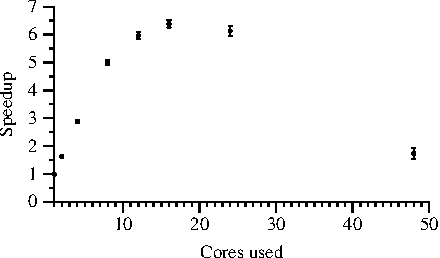
\includegraphics[width=2.8in]{speedup.pdf}}
   \caption{MRFy's parallel speedup on an 8-bladed $\beta$-propeller, using a
   48-core system.
   After about 12 cores, speedup falls off.}
   \label{speedup}
 \end{center}
\end{figure}

\subsection{Remote homology detection accuracy}

We performed cross-validation testing on 11 $\beta$-barrel superfamilies, both
with and without simulated evolution.
For MRFy, the balance between accuracy and computational efficiency is 
determined by the termination conditions, as well as the search technique 
chosen.
Because local search so dramatically outperformed simulated annealing and the
genetic algorithm, we conducted these cross-validation tests only on local 
search.
We chose 30 seconds as a balance between speed and accuracy; a 5 minute time
limit might result in better accuracy, but for high-throughput, whole-genome 
scans, 5 minutes per alignment is excessive.

We compared MRFy's performance, both with and without simulated evolution, to 
the results from \citet{Daniels:2012dg}.
Table~\ref{mrfy-auc} shows the area (AUC) under the Receiver Operator 
Characteristic (ROC) curve for MRFy, the very best result from SMURFLite, and
HMMER, RAPTOR, and HHPred.
Importantly, we are choosing the best SMURFLite parameters for each superfamily,
which could not be known in advance; thus, we demonstrate improvements over the
\emph{very best} SMURFLite can perform, rather than just an average case.

We first note the ``Barwin-like endoglucanases'' superfamily highlighted in
\citet{Daniels:2012dg}.
SMURFLite performed better as the interleave threshold was increased on this
superfamily, and also when simulated evolution was added.
Since MRFy discards no $\beta$-strands, we were curious how it would perform
on this superfamily.
Notably, this superfamily has exceedingly little training data; during 
cross-validation, there are at most 4 training sequences and as few as 3
when filtered at a BLAST E-value of $10^{-7}$ and the family under test is left
out.
Without simulated evolution, MRFy achieves an AUC of 0.86, outperforming 
SMURFLite
without simulated evolution (SMURFLite achieved an AUC of 0.77 with an 
interleave threshold of 2, and 0.81 with an interleave threshold of 4).
When simulated evolution is added, MRFy achieves an AUC of 0.92, outperforming
SMURFLite with an interleave threshold of 2, but falling just short of the 0.94
AUC SMURFLite demonstrates with an interleave threshold of 4 and simulated 
evolution.
We note that the running time required for SMURFLite with an interleave
threshold of 4 was roughly 10 minutes; MRFy required only 30 seconds to achieve
comparable results.

MRFy outperforms SMURFLite in terms of AUC on four of the $\beta$-barrel 
superfamilies, while SMURFLite outperforms MRFy on three.
There was only one superfamily, the ``Prokaryotic SH3-related domain,'' where
SMURFLite outperformed HMMER, RAPTOR, and HHPred while MRFy did not (MRFy, with 
an AUC of 0.73, fell behind HMMER's 0.81 AUC).
Unfortunately, MRFy never produced the best performance on a superfamily that 
SMURFLite had not performed best on in our previous work.
Thus, with the exception of the ``Barwin-like endoglucanase'' superfamily, the
added $\beta$-strand information does not seem to help MRFy significantly in 
the cases where HMMER, RAPTOR, or HHPred performed best.

%%%

\rowcolors{2}{gray!25}{white}

\newcolumntype{H}[1] {%
>{\raggedright}%
p{#1}}

\begin{small}

\begin{center}
\begin{table*}[!t]
\caption{AUC on Beta-Barrel superfamilies\label{mrfy-auc}}
{\footnotesize \begin{tabular*}{\textwidth}{@{\extracolsep{\fill}}H{3.3cm}p{1.0cm}p{1.1cm}p{1.0cm}p{2.4cm}p{0.7cm}p{1.6cm}p{1.6cm}}\hline
 & HMMER & RAPTOR & HHPred & SMURF\-Lite & MRFy$^{1}$ & MRFy$^{1}$, SE & MRFy$^{2}$\\
 \hline
{\bf MRFy performs best}  & & & & & & & \\
\hline
Translation proteins & - & - & 0.66 & 0.93 & {\bf 0.95} & 0.91 & {\bf 0.95}\\
Barwin-like endoglucanases & - & - & 0.75 & 0.77 & 0.86 & {\bf 0.92} & {\bf 0.94} \\
Tudor/PWWP/MBT & 0.78 & 0.74 & 0.67 & 0.83 & {\bf 0.86} & {\bf 0.86} & {\bf 0.86}\\
Nucleic acid-binding proteins & 0.75 & - & 0.67 & 0.89 & 0.75 & {\bf 0.95} & {\bf 0.95} \\
 \hline
 {\bf SMURFLite performs best}  & & & & & & & \\
\hline
Cyclophilin-like & 0.67 & 0.61 & 0.7 & {\bf 0.85} & 0.82 & 0.80 & {\bf 0.85} \\ 
Sm-like ribonucleoproteins & 0.73 & 0.71 & 0.77 & {\bf 0.85} & 0.77 & 0.77 & {\bf 0.87} \\
Prokaryotic SH3-related domain & 0.81 & -  & - & {\bf 0.83} & 0.73 & 0.72 & {\bf 0.84} \\
 \hline
{\bf HHPred performs best}  & & & & & & &\\
\hline
Translation proteins SH3-like & 0.83 & 0.81 & {\bf 0.86} & 0.62 & - & 0.63 & 0.63\\
 \hline
 {\bf RAPTOR performs best} & & & & & & \\
\hline
PDZ domain-like & 0.96 & {\bf 1.0} & 0.99 & 0.97 & 0.95 & 0.95 & 0.96 \\
FMN-binding split barrel & 0.62 & {\bf 0.82} & 0.61 & - & - & - & -\\
 \hline
{\bf HMMER performs best}  & & & & & & & \\
\hline
Electron Transport accessory proteins & {\bf 0.84} & - & 0.77 & 0.66 & - & 0.68  & 0.68\\
\hline
\end{tabular*}}\\{Note: for SMURFLite, value indicated is the best of all
values from~\cite{Daniels:2012dg}. For MRFy, SimEv is simulated evolution. A 
dash ('-') in a result entry indicates the method failed on these structures, 
i.e. an AUC of less than 0.6}
\end{table*}
\end{center}

\end{small}

\rowcolors{0}{white}{white}



\section{Discussion}

We have presented MRFy, a method that uses stochastic search to find 
alignments of protein sequences to Markov random field models.
MRFy outperforms SMURFLite in most cases, but we should consider several 
possible enhancements to MRFy that might improve its performance.
As demonstrated on the $\beta$-sandwich superfamily, MRFy with local search 
achieves a globally optimal alignment when given 5 minutes of run-time, but 
fails to find a score close to this when given only 30 seconds.
It was not immediately clear how to bring convergence testing into the local
search model, but doing so might achieve results comparable to the 5 minute
results in less time.

We hope that MRFy will be useful for whole-genome annotation of newly-sequenced
organisms.
The tradeoff of time versus accuracy suggests a two-phase approach to this task:
a scan with relatively strict run-time performance requirements (perhaps no more
than ten seconds per alignment) coupled with a relatively loose $p$-value 
threshold would produce a number of candidates, many of which would likely be
false positives.
Then, MRFy could be re-run on these candidates with more computationally
demanding settings, and with a more strict $p$-value threshold.
MRFy computes $p$-values identically to SMURFLite: an extreme value 
distribution~\cite{Eddy:1998ut} is fitted to a distribution of raw scores,
and then a $p$-value is computed as $1-cdf\left( x \right)$ for any raw MRFy 
score $x$.
Computing the $p$-value accurately in the face of different search intensities
might require fitting multiple distributions, each for a different level of
search intensity.
Otherwise, if the distribution is obtained with an intensive search, then at
less-intensive search parameters, true positives may result in poor $p$-values;
similarly, if the distribution is obtained with a quick search, then 
more-intensive search parameters might result in false positives scoring 
comparatively well, and appearing to have good $p$-values.

As in~\cite{Daniels:2012dg}, we compared MRFy to 
HHPred~\cite{Soding:2005ff}.
As discussed, HHPred has an advantage in that it builds profiles based on all
of protein sequence space.
As a future enhancement to MRFy, we plan to introduce query profiles, so that
the MRFy alignment is to a sequence profile built from the query sequence,
rather than just the query sequence.
However, this will introduce a run-time performance hit in two ways.
First, the time to run a sequence homology search using the BLAST~\cite{Altschul:1997tl} 
family of tools can be significant, though the work on 
compressively-accelerated algorithms by Loh, et al.\cite{Loh:2012br} may reduce this 
impact.
Second, computing the Viterbi and $\beta$-pairing scores na\"{i}vely will
require time directly proportional to the number of sequences in the query
profile.
Representing these query sequences as sets of residue frequency vectors should
help, and there may be other approaches to consider.

We have demonstrated that MRFy is an improvement to SMURFLite, one that brings
the full power of a Markov random field to bear.
Thus far, only $\beta$-strand interactions lead to non-local interactions in the
MRFy Markov random field.
In the future, we will investigate fitting other secondary structural elements
(the $\alpha$-helices) into this model.
In addition, disulfide bonds, which can occur between cysteine residues and
have been shown to be highly conserved~\cite{Naamati:2009eg, Tirosh:2012iq}, 
would appear to fit easily into this model.

\section{Acknowledgements}
Thanks to Richard Senington for the original local search implementation. 
This work was funded in part by NIH grant 1R01GM080330-01A1 (to L.C.).



{\small 
\bibliographystyle{abbrv}
\bibliography{mrfy}  }

\end{document}
